\documentclass[11pt,a4paper]{article}

\usepackage[margin=19mm]{geometry}
\usepackage{xcolor}
\usepackage{booktabs}
\usepackage{tabularx}
\usepackage{array}
\usepackage{tikz}
\usepackage{hyperref}
\usepackage{fancyhdr}
\usepackage{titlesec}
\usepackage{amsmath}

\definecolor{navy}{HTML}{17324D}
\definecolor{blue}{HTML}{2F80ED}
\definecolor{cyan}{HTML}{EAF6FF}
\definecolor{green}{HTML}{219653}
\definecolor{greenbg}{HTML}{EAF7EF}
\definecolor{amber}{HTML}{F2994A}
\definecolor{amberbg}{HTML}{FFF3E4}
\definecolor{graybg}{HTML}{F6F8FA}
\definecolor{textgray}{HTML}{4F5B67}

\hypersetup{colorlinks=true,urlcolor=blue,linkcolor=blue}
\pagestyle{fancy}
\fancyhf{}
\lhead{\textcolor{textgray}{Gemini Live Voice Usage Estimate}}
\rhead{\textcolor{textgray}{NDIS Onboarding Assistant}}
\cfoot{\thepage}

\titleformat{\section}{\large\bfseries\color{navy}}{\thesection}{0.7em}{}
\titleformat{\subsection}{\normalsize\bfseries\color{navy}}{\thesubsection}{0.7em}{}

\newcommand{\metricbox}[4]{
\begin{tikzpicture}
  \node[
    rounded corners=5pt,
    fill=#1,
    draw=#2,
    line width=0.7pt,
    inner sep=10pt,
    text width=#3
  ] {#4};
\end{tikzpicture}
}

\begin{document}

\begin{center}
{\Huge\bfseries\color{navy} Gemini Live Voice Usage Cost Estimate}\\[3mm]
{\large NDIS Structured Onboarding Voice Assistant}\\[4mm]
{\small Production planning estimate for internal/client discussion}
\end{center}

\vspace{5mm}

\section*{Executive Summary}

\metricbox{greenbg}{green}{0.94\textwidth}{
\textbf{The current A\$103 monthly Google Cloud bill should not be used as a fixed estimate for one normal organisation.}

\vspace{2mm}

The correct production estimate depends on total \textbf{active voice hours} across all organisations, providers, workers, and participants. Production cost may be lower, similar, or higher than A\$103 depending on adoption and real usage volume.
}

\vspace{4mm}

This assistant is a structured onboarding workflow, not an always-on chatbot. Users only consume Gemini Live voice usage while the voice session is active. Some participants may complete the workflow in one sitting, while others may complete it over several days. The calendar duration does not drive AI cost; total active voice time does.

\section*{Cost Basis}

For planning purposes, Gemini realtime voice usage is estimated using the following conservative range:

\begin{center}
\begin{tabularx}{0.88\textwidth}{>{\bfseries}l r}
\toprule
Planning Unit & Estimated Gemini Voice Cost \\
\midrule
Per active voice minute & A\$0.02--A\$0.04 \\
Per active voice hour & A\$1.20--A\$2.40 \\
\bottomrule
\end{tabularx}
\end{center}

\vspace{2mm}

\[
\textbf{Monthly Gemini Voice Cost}
=
\text{Total Active Voice Hours}
\times
\text{A\$1.20 to A\$2.40}
\]

\vspace{2mm}

\metricbox{cyan}{blue}{0.94\textwidth}{
\textbf{Important distinction:} A participant who takes one week to finish onboarding does not necessarily cost more than a participant who finishes in one day. The cost depends on how many minutes they actively use the voice assistant.
}

\section*{Usage Scenarios}

\begin{center}
\begin{tabularx}{0.95\textwidth}{>{\bfseries}l r r X}
\toprule
Scenario & Active Voice Time & Estimated Cost & Notes \\
\midrule
Fast completion & 10 minutes & A\$0.20--A\$0.40 & User answers quickly with minimal repeats. \\
Typical guided completion & 20 minutes & A\$0.40--A\$0.80 & Reasonable planning case for a guided flow. \\
Slower assisted completion & 45 minutes & A\$0.90--A\$1.80 & More pauses, repeats, or support needed. \\
Very slow / interrupted flow & 90 minutes & A\$1.80--A\$3.60 & Spread over one or more sessions. \\
\bottomrule
\end{tabularx}
\end{center}

\section*{Monthly Organisation-Level Examples}

The table below shows how monthly cost changes as total active voice usage increases. These examples are not per-person guarantees; they are usage-volume scenarios.

\begin{center}
\begin{tabularx}{0.92\textwidth}{>{\bfseries}r r r X}
\toprule
Total Active Voice Hours / Month & Low Estimate & High Estimate & Interpretation \\
\midrule
25 hours & A\$30 & A\$60 & Light usage / early pilot. \\
50 hours & A\$60 & A\$120 & Moderate usage; close to current A\$103 range. \\
100 hours & A\$120 & A\$240 & Higher adoption across users. \\
250 hours & A\$300 & A\$600 & Larger provider network or frequent usage. \\
500 hours & A\$600 & A\$1,200 & High-volume rollout. \\
\bottomrule
\end{tabularx}
\end{center}

\vspace{3mm}

\begin{center}
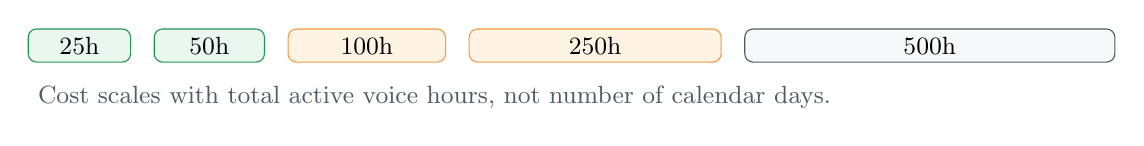
\begin{tikzpicture}
  \draw[fill=greenbg, draw=green, rounded corners=3pt] (0,0) rectangle (1.3,0.42);
  \node at (0.65,0.21) {\small 25h};
  \draw[fill=greenbg, draw=green, rounded corners=3pt] (1.6,0) rectangle (3.0,0.42);
  \node at (2.3,0.21) {\small 50h};
  \draw[fill=amberbg, draw=amber, rounded corners=3pt] (3.3,0) rectangle (5.3,0.42);
  \node at (4.3,0.21) {\small 100h};
  \draw[fill=amberbg, draw=amber, rounded corners=3pt] (5.6,0) rectangle (8.8,0.42);
  \node at (7.2,0.21) {\small 250h};
  \draw[fill=graybg, draw=textgray, rounded corners=3pt] (9.1,0) rectangle (13.8,0.42);
  \node at (11.45,0.21) {\small 500h};
  \node[anchor=west, text=textgray] at (0,-0.45) {\small Cost scales with total active voice hours, not number of calendar days.};
\end{tikzpicture}
\end{center}

\section*{Current A\$103 Bill Interpretation}

The current A\$103 monthly bill is best treated as a reference point from the development/testing period, not a direct production benchmark.

\begin{center}
\begin{tabularx}{0.94\textwidth}{>{\bfseries}l X}
\toprule
Observation & Interpretation \\
\midrule
Known development testing was approximately 16 hours & This is a limited internal testing sample, not representative of broad production usage. \\
Development testing differs from real usage & Testing includes repeated sessions, reconnects, debugging, and edge-case checks. \\
Production may involve many users & Total production cost can exceed testing if many providers and participants actively use voice. \\
Best estimate method & Forecast by expected active voice hours per month, then update after pilot telemetry. \\
\bottomrule
\end{tabularx}
\end{center}

\section*{Recommended Production Forecasting Method}

\begin{enumerate}
  \item Estimate expected monthly active voice hours.
  \item Multiply by A\$1.20--A\$2.40 per active voice hour.
  \item Review real usage after the first pilot month.
  \item Replace assumptions with measured session duration and usage data.
\end{enumerate}

\vspace{2mm}

\metricbox{amberbg}{amber}{0.94\textwidth}{
\textbf{Commercial position:} A\$103 is not automatically high or low. It is simply not enough information by itself. The production monthly cost will depend on how many organisations use the assistant and how many total active voice hours they generate.
}

\section*{Conclusion}

\begin{center}
\metricbox{greenbg}{green}{0.86\textwidth}{
\centering
\Large\bfseries
Use active voice hours as the pricing model.\\[1mm]
A\$103 is a reference point, not a fixed production estimate.
}
\end{center}

\end{document}
